\section{Softwarearchitektur}\label{sec:softwarearchitektur}

Die \textbf{Softwarearchitektur} beschreibt den grundlegenden Aufbau einer Softwarelösung.\\

\noindent
Dabei beantwortet eine Softwarearchitektur typische Fragen wie

\begin{itemize}
    \item wird die Anwendung auf einem Rechner ausgeführt oder auf mehreren?
    \item wenn sie auf mehreren Rechnern ausgeführt wird, wie wird die Anwendung dann verteilt?
    \item wie kommunizieren die Komponenten untereinander?
    \item wird eine Datenbank verwendet?
    \item wie sieht der Aufbau der Software in Gesamtsicht aus?
    \item welche Software /Frameworks kommen zum Einsatz?
    \item welche Strategie wird bei dem Ausfall einzelner Komponenten verfolgt?
\end{itemize}

\subsection*{Architektur am Anfang}
Die Beantwortung dieser Fragen hat entscheidende Auswirkungen auf die weitere Entwicklung der Software, deshalb sollten Softwarearchitekten bereits beteiligt sein, wenn es um die Klärung der \textbf{Geschäftsanforderungen} geht (s.a. Abschnitt~\ref{sec:lastenheft-vision-scope}).\\

\begin{figure}
    \centering
    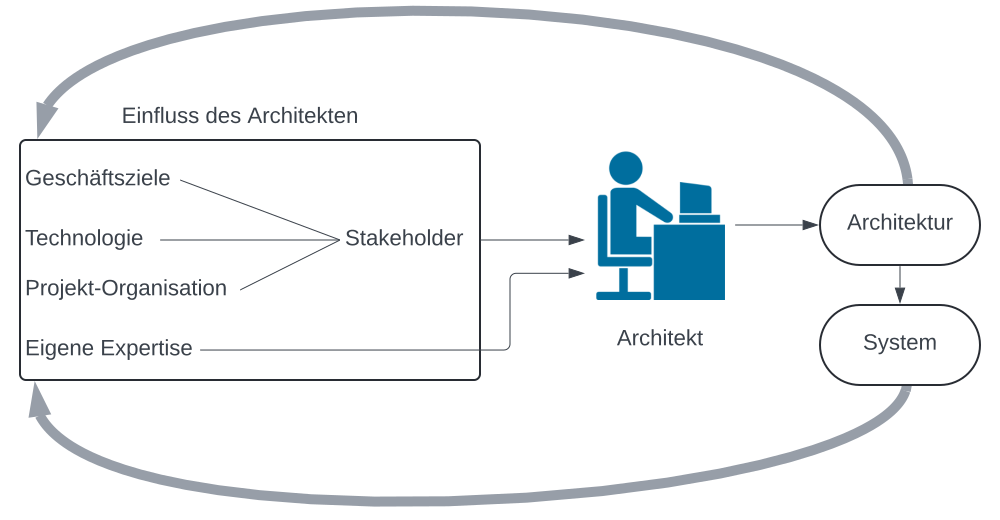
\includegraphics[scale=0.4]{part two/Architektur/img/aic}
    \caption{Der \textit{Architecture Influence Cycle} nach \textit{Bass, Clements, und Kazman}. Qualitäts-, Geschäfts- und organisatorische Anforderungen beeinflussen die Arbeit des Architekten, die wiederum diese Anforderungen beeinflussen können. Zusätzlich wirken eigene Erfahrungen auf seine Planung ein, die wiederum in ein Folgeprojekt einfließen können. (Quelle: in Anlehnung an~\cite[58, Figure 3.5]{BCK12})}
    \label{fig:aic}
\end{figure}


\noindent
Dabei liefern Architekten \textbf{Aufwandsabschätzungen}, die die Wirtschaftlichkeit beeinflussen können, und überprüfen die Machbarkeit von Ideen.\\
Hierbei entsteht eine \textbf{Rückkoppelungsschleife}, da Ideen zum Produkt zu Fragen und Aussagen zur Softwarearchitektur führen, die wiederum die Ideen zum Produkt beeinflussen (vgl.\cite[37]{Wed09b}, s. außerdem Abbildung~\ref{fig:aic}).

\subsection*{Grundlage: Anforderungen und Randbedingungen}
Grundlage für die Auswahl einer Softwarearchitektur sind die \textbf{Anforderungen} und \textbf{Randbedingungen}.

\vspace{2mm}
\begin{tcolorbox}
    Die Architektur muss so ausgestaltet werden, dass sie die Erfüllung der Anforderungen unter Einhaltung der Randbedingungen ermöglicht.\\
    In fast allen Fällen bestimmen nicht die funktionalen, sondern die nicht-funktionalen Anforderungen die Systemarchitektur.
\end{tcolorbox}
\vspace{2mm}

\noindent
Generell wird also zunächst festgestellt, welche Auswirkungen die Randbedingungen im Hinblick auf Vorgaben oder Einschränkungen haben, anschließend wird entsprechend ihrer \textit{Gewichtung} dafür gesorgt, dass die Architektur die nicht-funktionalen Anforderungen erfüllt.

\subsection*{Taktiken}
\textbf{Taktiken} sind \textbf{Standardlösungen}, wie eine Architektur auf grundlegende Art und Weise nicht-funktionale Anforderungen erfüllbar machen kann.\\
Unter \textit{Taktik} versteht man bspw., wie hoch-verfügbare Systeme strukturiert und gebaut werden können.

\subsection*{Referenzarchitekturen und Frameworks}
\textbf{Referenzarchitekturen} sind \textbf{Referenzmodelle}, die bei der Entwicklung einer Architektur hinzugezogen werden können, wie bspw. \textbf{Aktive Redundanz}\footnote{s. Glossar}.\\

\noindent
Diese werden häufig durch vorgefertigte Frameworks unterstützt bzw. realisiert.

\subsection*{Dokumentation in Sichten}
Architekturen werden in Sichten dokumentiert:

\begin{itemize}
    \item \textbf{Kontextsicht} (zeigt das System als Blackbox in seinem Kontext aus einer Vogelperspektive)
    \item \textbf{Baustein-Sicht} (statisches Modell: ``Bausteinsichten zeigen die statischen Strukturen der Architekturbausteine des Systems, Subsysteme, Komponenten und deren Schnittstellen.``\footnote{
        \cite[81]{Sta14e}.
        Nachfolgende Beschreibungen der Sichten wurden \textit{Starke} entnommen.
    } Dies beinhaltet auch die Organisation des Quellcodes.)
    \item \textbf{Laufzeitsicht} (dynamisches Modell, Zusammenwirken der Bausteine des Systems zur Laufzeit)
    \item \textbf{Verteilungssicht} (Beschreibung der Hardwarekomponenten, auf denen das System läuft; dokumentiert Rechner, Prozessoren, Netztopologien u.a., also Bestandteile der \textit{physischen} Systemumgebung: Das System wird aus Betreibersicht gezeigt)
\end{itemize}

\subsection*{Prove it with code}

\begin{tcolorbox}
    Eine Architektur soll nicht-funktionale Anforderungen erfüllen und grundlegende Strukturen beschreiben.
\end{tcolorbox}

\noindent
Damit Schwachstellen einer Architektur nicht erst nach Fertigstellung einer Software deutlich werden, sollte diese zumindest mit einem sehr einfachen Prototypen erprobt werden.
Hierdurch kann im Sinne der \textbf{Qualitätssicherung} der Ansatz ausprobiert werden, und im Sinne der \textbf{Dokumentation} den Entwicklern eine Musterimplementierung zur Verfügung gestellt werden.